% !TeX spellcheck = de_DE
\setcounter{section}{1} % Somit ist STL immer 2.x auch ohne THD
%	\setlength{\abovedisplayskip}{0pt}
%	\setlength{\belowdisplayskip}{0pt}
%	\setlength{\abovedisplayshortskip}{0pt}
%	\setlength{\belowdisplayshortskip}{0pt}

\section{Strömungslehre}
	Dazu gehört auch die THD Formelsammlung. Notiz: $ \text{rho} = \varrho \neq p = \text{Druck}, \ \text{nü} = \nu \neq v  $

\subsection{Hydrostatik}

	\begin{flushleft}
		\setlength{\tabcolsep}{1.5em} % for the horizontal padding
		{\renewcommand{\arraystretch}{1.5}
		\begin{tabular}{ll}
			\multicolumn{2}{l}{$ i $ kennzeichnet eine beliebige Richtung z.B. $ x,\, y,\, z $ oder die Richtung einer schrägen Wand $ s $}                                  \\
			\multicolumn{2}{l}{$ S $ kennzeichnet den Schwerpunkt}                                                                                                           \\
			Druckgradient: $ \dfrac{\partial p}{\partial x_i} =  \varrho\ f_i$ & Für $ f_z = g $ ist der Überdruck $ p_{\ue(z)} =  \varrho\ g\ z \quad \ g,\, z \downarrow $ \\
			Exzentrizität:       $ e_{Si} = \dfrac{I_{Si}}{s_{Si} \ A}$        & Vertikale Wandkraft: $ F_{wi} = p_{\ue,S} \ A_i $                                           \\
			\multicolumn{2}{l}{$ s_{Si} $ Lage des Flächenschwerpunkts $ S $ von Oberfläche in Richtung $ i $}                                                               \\
			\multicolumn{2}{l}{$ I_{Si} $ Flächenträgheitsmoment in Richtung $ i $ um horizontale Achse durch Schwerpunkt $ S $ }                                            \\
			\multicolumn{2}{l}{Horizontale Wandkraft 	$ F_{wz} $ = Gewicht des darüberliegenden Fluids}
		\end{tabular}
		}
	\end{flushleft}
%
	\vspace{-0.8cm}
%
	\begin{center}
		\setlength{\tabcolsep}{0.5em} % for the horizontal padding
		{\renewcommand{\arraystretch}{1.7}
		\begin{tabular}{llll}
			Rechteckiger Deckel mit Breite a, Höhe b:              & $ I_{Ss} = \dfrac{a\ b^3}{12} $  & $ A = a \ b $                                             & $ e_{Ss} = \dfrac{b^2}{12\ s_{Ss}} $            \\
			Kreisförmiger Deckel mit Radius r:                     & $ I_{Ss} = \dfrac{r^4\ \pi}{4} $ & $ A = r^2 \ \pi $                                         & $ e_{Ss} = \dfrac{r^2}{4\ s_{Ss}} $             \\
			Gleichschenkeliges Dreieck, Basis a, Höhe b:           & $ I_{Ss} = \dfrac{a\ b^3}{36} $  & $ A = \dfrac{a \ b}{2} $                                  & $ e_{Ss} = \dfrac{b^2}{18\ s_{Ss}} $            \\
			\multicolumn{4}{l}{Statische Auftriebskraft an der Unterseite eines eingetauchten Körpers:  $ F_A = \varrho_{Fl} \ g \ V_{K,eingetaucht} $ }                                                            \\
			Horizontal beschleunigte Flüssigkeiten:                & \multicolumn{2}{l}{$ p_{\ue(x,z)} = -\varrho\ a\ x - \varrho\ g\ (z-z_0) $}                  & $ z_0 = h_0 + \dfrac{a}{g} x_S $                \\
			\qquad Spiegeloberfläche                               & \multicolumn{2}{l}{ Neigung $ \alpha = \arctan \dfrac{a}{g} $}                               & $ z_{(x)} = z_0 - \dfrac{a}{g} x $              \\
			Rotierend beschleunigte Flüssigkeiten:                 & \multicolumn{2}{l}{$ p_{\ue(r,z)} = \dfrac{\varrho}{2}\ r^2\ \omega - \varrho\ g\ (z-z_0) $} & $ z_0 = h_0 - \dfrac{I_p\ \omega^2}{2\ g\ A} $  \\
			\qquad Spiegeloberfläche                               & \multicolumn{2}{l}{$ I_p = I_{pS} + r_S^2\ A $}                                              & $ z_{(r)} = z_0 + \dfrac{r^2\ \omega^2}{2\ g} $ \\
			 \multicolumn{4}{l}{$ I_{pS} $ polare Trägheitsmoment um Schwerpunkt $ S $ \quad $ r_S $ ist der Abstand vom Schwerpunkt zur Drehachse}
		\end{tabular}
		}
	\end{center}

\subsection{Aerostatik}
	\skipabove{-10pt}
	\[
		\text{Standardatmosphäre } \nn =  \num{1.235}
		\qquad  \po = \qty{1}{atm} = \qty{101325}{\Pa}
		\qquad  \To = \qty{15}{\degreeCelsius} = \qty{288,15}{\K}
		\qquad  \Ho = \qty{8430}{\m}
	\]
	\[
	  		   \dfrac{p_{(z)}}{\po} = \left( 1 - \dfrac{\nn-1}{\nn}  \dfrac{z}{\Ho} \right) ^{\dfrac{\nn}{\nn-1}}
	 	\qquad \dfrac{T_{(z)}}{\To} = \left( 1 - \dfrac{\nn-1}{\nn}  \dfrac{z}{\Ho} \right)
	  	\qquad \dfrac{\varrho_{(z)}}{\varrho_0} = \left( 1 - \dfrac{\nn-1}{\nn}  \dfrac{z}{\Ho} \right) ^{\dfrac{1}{\nn-1}}
	\]

\subsection{Massenbilanz MB}
	\skipabove{-15pt}
	\[
		\sum \dot{m}_{ein} - \sum \dot{m}_{aus} = 0
		\qquad  \dot{m} = \varrho\ \dot{V}
		\qquad  \dot{V} = A\ c
		\qquad  c \perp A
 	\]

\subsection{Energiebilanz EB, siehe auch THD}
	\skipabove{-15pt}
	\[ \arraycolsep=0em\def\arraystretch{1.7}
	\begin{array}{l p{4em} l}
		\Delta h + \Delta \dfrac{c^2}{2} + g\ \Delta z = \Delta q_a + \Delta w_i     & & \Delta h = \Delta q_a + \Delta q_R + \int v\ \dd p                                                         \\
		\int v\ \dd p + \Delta q_R + \Delta \dfrac{c^2}{2} + g\ \Delta z = \Delta w_i& & \text{Inkompressibel: } \dfrac{\Delta p}{\varrho} + \Delta q_R + \Delta \dfrac{c^2}{2} + g\ \Delta z = \Delta w_i
	\end{array} \]

\clearpage
\subsection{Impulsmomentenbilanz um Achse \textit{i} $\mathbf{IB_i}$ }
	$ c_i $ ist die Geschwindigkeitskomponente in Richtung $ i $ (relativ zum bewegten Kontrollvolumen)
%
	\begin{center}
		\setlength{\tabcolsep}{0.65em} % for the horizontal padding
		\begin{tabular}{lllll}
			  $ \sum \dot{I}_{ein} - \sum \dot{I}_{ein} + \sum F_{p,i} + \sum F_{R,i} + \sum F_{g,i} = 0$
			& $ \dot{I} = \dot{m} \ c_i $
			& $ F_{p,i} = p_{\ue} \ A_i $
			& $ F_{R,i} = \tau_W \ A_{Wi} $
			& $ F_{g,i} = m \ g_i $
		\end{tabular}
	\end{center}

\subsection{Impulsbilanz in Richtung \textit{i} $\mathbf{IB_i}$ }
	$ c_n $ ist die Geschwindigkeit projiziert auf die Normalebene der Achse $ i $

	$ r_i $ ist der Hebelarm zur Achse $ i $ in der Normalebene der Achse $ i $
%
	\begin{center}
		\setlength{\tabcolsep}{0.36em} % for the horizontal padding
		\begin{tabular}{lllll}
			$ \sum \dot{L}_{ein} - \sum \dot{L}_{ein} + \sum M_{p,i} + \sum M_{R,i} + \sum M_{g,i} = 0$
			& $ \dot{L} = \dot{m} \ c_n \ r_i $
			& $ M_{p,i} = F_p\ r_i $
			& $ M_{R,i} = F_R\ r_i $
			& $ M_{g,i} = F_g\ r_i $
		\end{tabular}
	\end{center}

\subsection{Isentrope kompressible Strömungen}
	Isentrope, ideales Gas, Isentropen-Koeffizient $\kappa$: Siehe THD Formelsammlung

	Index $ T $ kennzeichnet totale Bedingungen bzw. Ruhebedingungen bei $ c = 0 $

	Index $ k $ kennzeichnet kritische Bedingungen bei Schallgeschwindigkeit $ c = a $

	Index $ u $ kennzeichnet Umgebungsbedingungen
%
	\skipabove{0pt}
		\[ \arraycolsep=2em\def\arraystretch{2}
		\begin{array}{ll}
			  \text{Geschwindigkeitsfunktion }  \nu & \text{Durchflussfunktion }  \psi
			\\
			   \nu_{(\frac{p}{p_T},\kappa)} =
			  	\sqrt{\dfrac{\kappa}{\kappa-1}
			  		\left[1 -
			  			\left(\dfrac{p}{p_T}\right)
			  				^{\frac{\kappa-1}{\kappa}}
			  		\right]}
			&  \psi_{(\frac{p}{p_T},\kappa)} =
				\sqrt{ \dfrac{\kappa}{\kappa-1}
					\left[
						\left(\dfrac{p}{p_T}\right)
							^{\frac{2}{\kappa}}
							-
						\left(\dfrac{p}{p_T}\right)
							^{\frac{\kappa+1}{\kappa}}
					\right]}
			\\
			  \text{EB: } c = \displaystyle\sqrt{2\ R\ T_T} \cdot \nu_{(\nicefrac{p}{p_T},\kappa)}
			& \text{MB: } \dot{m} = A\ \varrho_T\ \displaystyle\sqrt{2\ R\ T_T} \cdot \psi_{(\nicefrac{p}{p_T},\kappa)}
		\end{array}\]
%
	\skipabove{0pt}
	\[
		\dfrac{p_k}{p_T} =
			\left(\dfrac{2}{\kappa+1}\right)
				^{\frac{\kappa}{\kappa-1}}
	\quad
		\nu_k = \sqrt{\dfrac{\kappa}{\kappa+1}}
	\quad
		\psi_k = \psi_{max} =
			\sqrt{\dfrac{\kappa}{\kappa+1}}
			\left(\dfrac{2}{\kappa+1}\right)
				^{\frac{1}{\kappa-1}}
	\quad
		\dfrac{T_k}{T_T} = \dfrac{2}{\kappa + 1}
	\quad
		\dfrac{\varrho_k}{\varrho_T} =
			\left(\dfrac{2}{\kappa+1}\right)
				^{\frac{1}{\kappa-1}}
	 \]
%
	\[
		c_k = a_k = \sqrt{\kappa \ R\ T_k}
	\qquad
		\text{Schallgeschwindigkeit: }
		a = \sqrt{\dfrac{\dd p}{\dd\varrho}}
			= \sqrt{\kappa \ R\ T}
	\qquad
		\text{Machzahl: }
		\Mach = \dfrac{c}{a}
	 \]

	Der Druck am Auslass einer einfachen konvergenten Düse $ p_a = \max(p_u, p_k) $

	Für gegebene Ruhebedingungen ist der Druck am Auslass einer korrekt ausgelegten Laval Düse $ p_a = p_u  $
%
	\skipabove{10pt}
	\[ \arraycolsep=2em\def\arraystretch{2}
	\begin{array}{ll}
		\Mach  =
		\sqrt{\dfrac{2}{\kappa-1}
			\left[\left(
				\dfrac{p}{p_T}
				\right)
					^{\frac{\kappa-1}{- \kappa}} - 1
			\right]}
		&
		\dfrac{p}{p_T}  =
			\left( 1 +
				\dfrac{\kappa-1}{2}  \Mach^2
			\right)
				^{\frac{- \kappa}{\kappa - 1}}
	\\
		\dfrac{\varrho}{\varrho_T}  =
		\left( \dfrac{p}{p_T} \right)
			^{\frac{1}{\kappa}} =
		\left( 1 +
			\dfrac{\kappa - 1}{2}  \Mach^2
		\right)
			^{\frac{- 1}{\kappa - 1}}
		&
		\dfrac{T}{T_T}  =
		\left( \dfrac{p}{p_T} \right)
			^{\frac{\kappa-1}{\kappa}} =
		\left( 1 +
			\dfrac{\kappa-1}{2}  \Mach^2
		\right)
			^{-1}
	\end{array}\]

\subsection{Viskosität -- Wandschubspannung}
	\begin{center}
		\setlength{\tabcolsep}{2em} % for the horizontal padding
		\begin{tabular}{ll}
		      Dynamische Viskosität $ \mu \text{ in } \left[\unit{\kg\per\m\per\s}\right] \text{ bzw. } \left[\unit{\Pa\s}\right] $
			& Kinematische Viskosität $ \nu = \dfrac{\mu}{\varrho} \text{ in } \left[\unit{\m\squared \per\s}\right] $
			\\
			  Newton'sches Schubspannungsgesetz $ \tau_{\textsl{w}} = \mu \dfrac{\dd c}{\dd y} $
			& $\gamma$ zeigt weg von der Wand.
		\end{tabular}
	\end{center}

\subsection{Durchströmung}
	\setlength{\abovedisplayskip}{-15pt}
	\[ \arraycolsep=0.7em
		\begin{array}{llll}
			N\!P\!S\!H = \dfrac{p - p_d}{\varrho\ g} & \dot{V} = c_{(y \text{ oder } r)} \ \dd A                                                    & \text{Kanal: } \dd A = b\ \dd y                                          & \text{Rohr: } \dd A = r\ \dd r\ \dd\varphi \\
			\text{Reynolds Zahl:}                    & \Reyn = \dfrac{\overline{c}\ L_{char}\ \varrho}{\mu} = \dfrac{\overline{c}\ L_{char}\ }{\nu} & L_{char} = d_h = \dfrac{4\ A}{U}                                         &                                             \\
			\text{Reibung:}                          & \Delta q_R = \dfrac{\Delta p_v}{\varrho} = g\ \Delta h                                       & = \left( \zeta_F + \lambda \dfrac{L}{d_h} \right) \dfrac{\overline{c}^2}{2} & \Delta p_v = R_{ges}\ \dot{V}^2             \\
			\text{Widerstand:}                       & R_i = \dfrac{\varrho}{2}  \left( \zeta_{Fi} + \lambda_i \dfrac{L_i}{d_{hi}}\right)              & \text{Seriell: } R_{ges} = \sum R_i  & \text{Parallel: } \dfrac{1}{R_{ges}} = \left[\sum\sqrt{\dfrac{1}{R_j}}\right]^2
		\end{array}
	\]
\subsection{Laminare Durchströmung}
	$ \Reyn_{dh} < 2300 $ \quad	Rohrreibungsbeiwert $ \lambda = \dfrac{64}{\Reyn_{dh}} $ \qquad	Hydrodynamische Einlaufstrecke $ \dfrac{L_e}{d_h} = \num{0,06} \Reyn_{dh}  $

	\skipabove{-5pt}
	\[ \arraycolsep=0em
	\begin{array}{l p{0.7em} l p{1.5em} l p{1.5em} l p{1.5em} l} % ich mag es nicht aber sonst indent :/
		\text{Couette Strömung:} && \dfrac{c_{(y)}}{c_{max}} = \dfrac{y}{h}                                                            && c_{max} = konst.                                       && A = b\ h     && \overline{c} = \dfrac{1}{2} c_{max} \\
		\text{Kanal Strömung:}   && \dfrac{c_{(y)}}{c_{max}} = 4 \left[\left(\dfrac{y}{h}\right) - \left(\dfrac{y}{h}\right)^2 \right] && c_{max} = \dfrac{1\ \Delta p_v\ h^2}{\mu\ \Delta L\ 8} && A = b\ h     && \overline{c} = \dfrac{2}{3} c_{max} \\
		\text{Rohr Strömung:}    && \dfrac{c_{(r)}}{c_{max}} = 1 - \left(\dfrac{r}{R}\right)^2                                         && c_{max} = \dfrac{1\ \Delta p_v\ R^2}{\mu\ \Delta L\ 4} && A = R^2\ \pi && \overline{c} = \dfrac{1}{2} c_{max}
	\end{array}
	\]
\subsection{Turbulente Durchströmung}
	$ \Reyn_{dh} > 4000 $ \quad	Rohrreibungsbeiwert $ \lambda $ aus Moody Diagr. \qquad	Hydrodynamische Einlaufstrecke $ \dfrac{L_e}{d_h} = \dfrac{8}{\sqrt{\lambda}}  $

	$ \nicefrac{1}{7} $ Potenzgesetz: $ \dfrac{c_{(r)}}{c_{max}} = 1 - \left(\dfrac{r}{R}\right)^{\nicefrac{1}{7}} $

\subsection{Strömungsmaschinen}
%
	\begin{flushleft}
		\setlength{\tabcolsep}{1.3em} % for the horizontal padding
		\begin{tabular}{lll}
			Drehzahl $ \dot{n} $                     & \multicolumn{2}{l}{Winkelgeschwindigkeit $ \omega = 2\ \pi\ \dot{n} $}                              \\
			Umfangsgeschwindigkeit $ u = r\ \omega $ & Relativgeschwindigkeit $ w $                       & Absolutgeschwindigkeit $ c $ \\
			Index $ r $ steht für Radialkomponente   & \multicolumn{2}{l}{Index $ u $ steht für Umfangskomponente}
		\end{tabular}
	\end{flushleft}

	\skipabove{-10pt}
		\[\arraycolsep=0.1em %\def\arraystretch{2}
		\begin{array}{ll}
			\text{MB: } \dot{m} = \varrho\ A_1\ c_{1r} = \varrho\ A_2\ c_{2r}                       & \text{EB: } \Delta p = \varrho\left[ \Delta w - \frac{1}{2} (c_2^2 - c_1^2) - \Delta q_R\right] \\
			\text{Euler'sche Momentengleichung aus IMB um Drehachse: }                              & M_{Antrieb} = \dot{m} (c_{2u}\ r_2 - c_{1u}\ r_1)                                               \\
			\text{Leistung: } P = M_{Antrieb}\ \omega = \dot{m}\ \Delta w                           & \text{Spez. Stutzenarbeit: } \Delta w = c_{2u}\ u_2 - c_{1u}\ u_1  (= Y)                        \\
			\text{Serienschaltung: } \dot{V} = \dot{V}_i   \qquad\qquad   \Delta p = \sum\Delta p_i & \text{Parallelschaltung: } \dot{V} = \sum\dot{V}_i   \qquad\qquad   \Delta p = \Delta p_i
		\end{array} \]

\subsection{Umströmung}
	Umschlag von laminar auf turbulent bei $ \num{5e5} < \Reyn_{Lchar} < \num{1e6} $

	Widerstandskraft $ F_W = c_W \dfrac{\varrho_{fl}}{2} c_{rel}^2\ A $ \qquad $ c_{rel} = c_{\infty} - c_{K\oum rper}$

\subsection{Umströmung einer Platte}
	Char. Länge $ L_{char} $ = Umströmte Plattenlänge $ L $ bzw. an der Stelle $ x $

	Bezugsfläche $ A = b\ L $ = Plattenoberfläche

	Einfluss der Rauigkeit: siehe Widerstandsdiagramm der Platte

	\[ \arraycolsep=1em\def\arraystretch{1.7}
	\begin{array}{|l|r|c|c|}
		\hline
		\quad                     & \quad                                                    & \text{Laminare Grenzschicht}  & \text{Turbulente Grenzschicht (glatt)} \\ \hline
		\text{Grenzschichtdicke}  & \dfrac{\delta}{x}                                      = & \dfrac{5}{\sqrt{\Reyn_x}}     & \dfrac{0,37}{\sqrt[5]{\Reyn_x}}        \\ \hline
		\text{Verdrängungsdicke}  & \dfrac{\delta_1}{x}                                    = & \dfrac{1,72}{\sqrt{\Reyn_x}}  & \dfrac{0,046}{\sqrt[5]{\Reyn_x}}       \\ \hline
		\text{Impulsverlustdicke} & \dfrac{\delta_2}{x}                                    = & \dfrac{0,665}{\sqrt{\Reyn_x}} & \dfrac{0,036}{\sqrt[5]{\Reyn_x}}       \\ \hline
		\text{Wandschubspannung}  & \dfrac{\tau_{\textsl{w}}}{\varrho \cdot u^2_{\infty}}  = & \dfrac{0,332}{\sqrt{\Reyn_x}} & \dfrac{0,0296}{\sqrt[5]{\Reyn_x}}      \\ \hline
		\text{Widerstandsbeiwert} & c_{\textsl{w}}                                         = & \dfrac{1,328}{\sqrt{\Reyn_l}} & \dfrac{0,074}{\sqrt[5]{\Reyn_l}}       \\ \hline
	\end{array} \]

	\clearpage
\subsection{Umströmung stumpfer Körper}
	\begin{doublespace}
		Char. Länge $ L_{char} $ = Hydraulischer Durchmesser der Schattenfläche in Strömungsrichtung

		Bezugsfläche $ A $ = Schattenfläche in Anströmrichtung

		Umströmungsgeschwindigkeit an dickster Stelle (Apex): Zylinder: $ c_{Apex}= 2\ c_{rel} $\quad Kugel: $ c_{Apex}= 1,5\ c_{rel}  $
	\end{doublespace}
	\vspace{-0.8em}
\subsection{Dynamischer Auftrieb}
	\begin{doublespace}
		Char. Länge $ L_{char} $ = Sehnenlänge des Profils $ L $

		Bezugsfläche $ A $ = Grundfläche des Profils bei Anstellwinkel $ \alpha = \qty{0}{\degree} $
	\end{doublespace}

	\[\arraycolsep=0.9em % for the horizontal padding
		\begin{array}{llll}
			\text{Dyn. Auftriebskraft }                          & \text{Kraft am Profilende}                           & \text{Nickmoment um Nase} & \text{Gleitzahl } \epsilon \text{ und Gleitwinkel } \gamma  \\
			F_A = c_A\ \dfrac{{\varrho}_{fl}} {2}\ c_{rel}^2 \ A & F_M = c_M\ \dfrac{{\varrho}_{fl}} {2}\ c_{rel}^2 \ A & M_N = F_M\ L              & \epsilon = \tan\gamma = \dfrac{F_W}{F_A} = \dfrac{c_W}{c_A}
		\end{array} \]

\subsection{Kompressible Flüssigkeiten}
	\skipabove{-25pt}
	\[\arraycolsep=0.2em \def\arraystretch{1.5}
	\begin{array}{lr p{2em} ll}
		\text{Schallgeschwindigkeit:}  & a = \sqrt{\dfrac{E}{\varrho}}  &  & \text{Flüssigkeit in elastischen Rohren:} & a = \dfrac{\sqrt{\dfrac{E}{\varrho}}} {\sqrt{1+ \dfrac{d\ E}{s\ E_R}}} \\
		\text{Empfohlene Schließzeit:} & \Delta t > 3\, \dfrac{2\ L}{A} &  & \text{Joukowski Stoß:}                    & \Delta p = \varrho\ a\ c
	\end{array} \]

\subsection{Gas-Flüssig Strömung}
	\setlength{\abovedisplayshortskip}{-20pt}
	\[\arraycolsep=0.3em \def\arraystretch{2}
	\begin{array}{lrclr}
		\text{Überdruck in Tröpfchen:}  & \Delta p = \dfrac{4\ \sigma}{d}                 & \text{\qquad} & \text{Spez. Zerstäubungsarbeit:} & \Delta w = \dfrac{6\ \sigma}{\varrho\ d} \\
		\text{Steighöhe in Kapillaren:} & h =  \dfrac{4\ \sigma\cos\gamma}{\varrho\ g\ d} & \text{\qquad} & \text{Weber Zahl:}               & \Webe = \dfrac{\varrho\ c^2\ d}{\sigma}  \\
		\text{Schallgeschwindigkeit:}   & a = \sqrt{\dfrac{\dd p}{\dd \varrho}}           & = &\multicolumn{2}{l}{ \sqrt{\dfrac{p_0\ \kappa\ \varrho_{g0}}{w_g\ \varrho^2}   \left[\dfrac{\varrho_{g0}}{w_g}  \left(\dfrac{1}{\varrho} - \dfrac{1-w_g}{\varrho_l}\right)\right] ^ {-\kappa-1}} }
	\end{array} \]
\subsection{Senkrechter Verdichtungsstoß}
	\setlength{\abovedisplayskip}{-15pt}
		\[ \arraycolsep=0.5em \def\arraystretch{2.5}
		\begin{array}{llp{1em}ll}
			\text{EB: } \dfrac{c_2}{c_1} = \dfrac{1}{\kappa+1}  \left[ \kappa - 1 + \dfrac{2}{\Mach_1^2}\right]                                    & < 1 &  & \text{IB: } \dfrac{p_2}{p_1} = 1+ \dfrac{2\ \kappa}{\kappa+1} (\Mach_1^2 - 1)                   & > 1 \\
			\text{MB: } \dfrac{\varrho_2}{\varrho_1} = \dfrac{(\kappa+1)\Mach_1^2}  {(\kappa-1)\Mach_1^2 + 2}                                      & > 1 &  &                                                                                                 &     \\
			\text{Mit: }  T = \dfrac{p}{R\ \varrho} \text{ und } a = \sqrt{\kappa\ R\ T} \text{ folgt: }                                           &     &  &                                                                                                 &     \\
			\dfrac{T_2}{T_1} = \dfrac{a_2^2}{a_1^2} = 1 +\dfrac{2\ (\kappa-1)}{(\kappa+1)^2}  \dfrac{\kappa \Mach_1^2+1}{\Mach_1^2}  (\Mach_1^2-1) & > 1 &  &                                                                                                 &     \\
			\Mach_2 = \dfrac{c_2}{a_2} = \sqrt{\dfrac{(\kappa-1) \Mach_1^2 + 2}{2\ \kappa\Mach_1^2 - (\kappa-1)}}                                  &     &  & \Delta s = s_2 - s_1 = c_p \ln\dfrac{T_2}{T_1} - R \ln\dfrac{p_2}{p_1}                          & >0  \\
			\text{Neue Ruhebedingungen nach dem Stoß:}                                                                                             &     &  & \dfrac{p_2}{p_{T2}} = \left( 1+ \dfrac{\kappa -1}{2}\Mach_2^2\right) ^{\frac{\kappa}{1-\kappa}} &
		\end{array} \]

\subsection{Schräger Verdichtungsstoß - Verdünnungswellen}
	\setlength{\abovedisplayshortskip}{-15pt}
	\[\arraycolsep=0.5em \def\arraystretch{2}
	\begin{array}{lc}
		\dfrac{c_2}{c_1}             = \dfrac{\cos\alpha_1}{\cos(\alpha_1-\delta)}                                                 & \multirow{5}{0.4\linewidth}{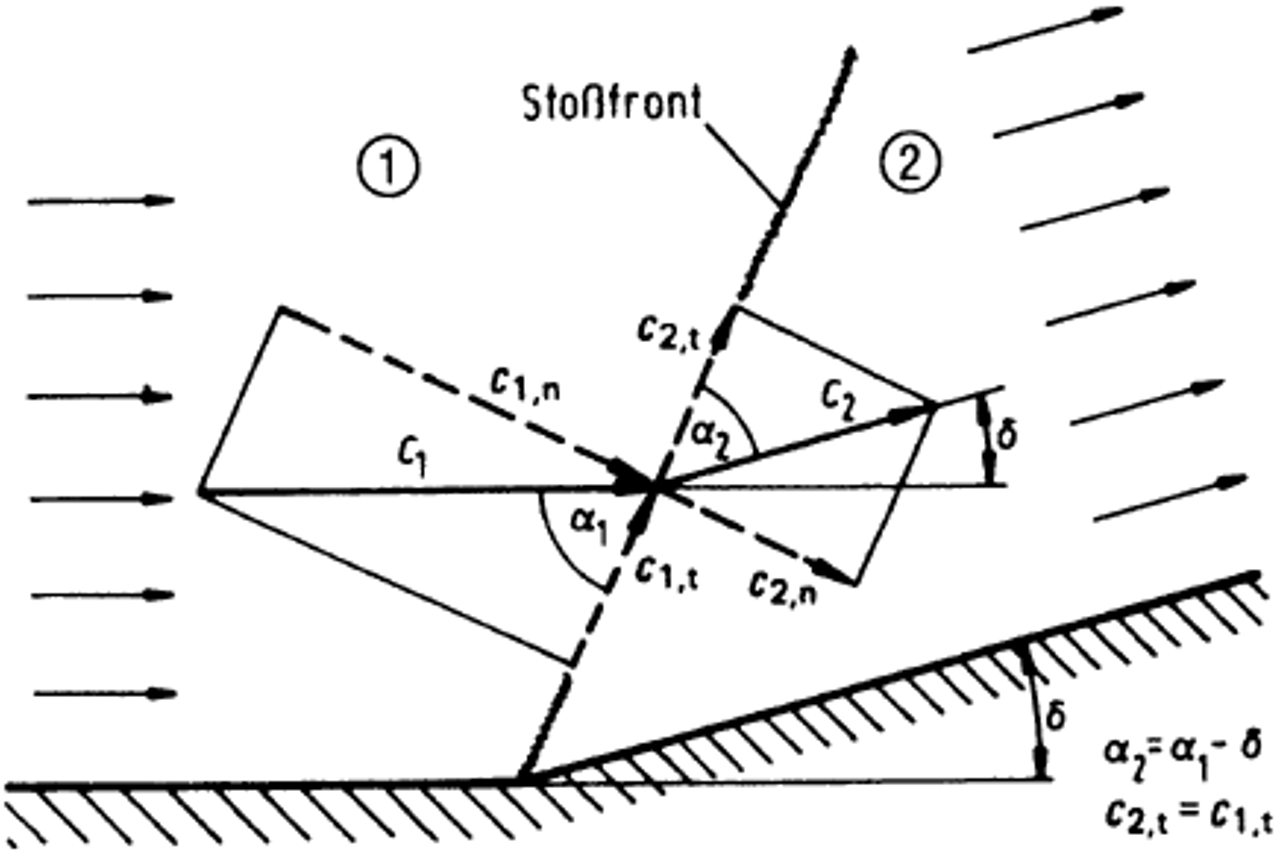
\includegraphics[width=\linewidth]{graphics/Verdichtungsstoss}} \\
		\dfrac{\varrho_2}{\varrho_1} = \dfrac{\tan\alpha_1}{\tan(\alpha_1-\delta)}                                                 &                                                                                             \\
		\dfrac{p_2}{p_1} = 1 + \dfrac{2\ \kappa}{\kappa + 1} \left[\left(\Mach_1\ \sin\alpha_1\right)^2 -1\right]                  &                                                                                             \\
		\cot\delta = \tan\alpha_1 \left[ \dfrac{\kappa+1}{2} \dfrac{\Mach_1^2}{\left(\Mach_1\ \sin\alpha_1\right)^2 -1} -1 \right] & \\
		\text{\quad} &
	\end{array} \]

\subsection{Erweiterungen zu Laval-Düse}
	Index $ a \dots $ Auslass;  $ k \dots $ kritischer/engster Querschnitt;  $ \alpha $ Winkel der Düse, bezogen auf Strömungsrichtung

	\skipabove{-5pt}
	\[
		\dfrac{A_a}{A_k} = \dfrac{1}{\Mach}  \left[ 1 + \dfrac{\kappa - 1}{\kappa + 1} \left( \Mach^2 -1 \right) \right] ^{\dfrac{\kappa + 1}{2\ (\kappa - 1)}}
		\qquad
		L = \dfrac{D_a - D_k}{2 \tan\alpha}
		\qquad
		\dfrac{\psi_a}{\psi_k} =  \dfrac{A_k}{A_a}
	\]

\subsection{Näherungen}
	\[ \arraycolsep=0.5em \def\arraystretch{2}
		\begin{array}{ll}
			\text{Abschätzung Reynolds}\Reyn > 1300 \dfrac{d}{k_s}
			\\
			\text{Näherung Rohrreibung } 65 \dfrac{d}{k_s} < \Reyn < 1300 \dfrac{d}{k_s}
			 &\rightarrow \
			\lambda_{Näherung} = \dfrac{0,25}{\left[\log\left(  \dfrac{15}{\Reyn} + \dfrac{k_s}{3,715\ d}  \right)\right]^2}
		\end{array}
	\]
	
\subsection{Energiebilanz – Ähnlichkeit}
	\begin{equation*}
		\dfrac{\Delta p}{\varrho \ c_{12}^2}
		+
		\dfrac{1}{2} \sum \left( 
			\zeta + \lambda_i \dfrac{l_i}{d_i} 
			\right)	\cdot 
			\dfrac{c_i^2}{2 \ c_{12}^2}
		+
		\dfrac{1}{2} \Delta \left( \dfrac{c}{c_{12}}^2 \right)
		+
		g \ \dfrac{L_{12}}{c_{12}^2} \cdot \dfrac{\Delta z}{L_{12}}
		=
		\dfrac{u_a^2}{c_{12}^2} \cdot \dfrac{\Delta w}{u_a^2}
	\end{equation*}
	
	\noindent
	$u_a$ \dots Umfangsgeschwindigkeit der Schaufel\\
	$A$ \dots Eulerzahl\\
	$B$ \dots Reynoldszahl + geometrische Ähnlichkeit
	$C$ \dots 